\documentclass[12pt,a4paper]{article}

% ---------------------------
% Pacotes essenciais
% ---------------------------
\usepackage[utf8]{inputenc}
\usepackage[T1]{fontenc}
\usepackage[brazil]{babel}
\usepackage{helvet}
\renewcommand{\familydefault}{\sfdefault}

\usepackage{geometry}
\usepackage{setspace}
\usepackage[table]{xcolor}
\usepackage{titlesec}
\usepackage{fancyhdr}
\usepackage{longtable}
\usepackage{tabularx}
\usepackage{array}
\usepackage{indentfirst}
\usepackage{hyperref}
\usepackage{enumitem}
\usepackage{ragged2e}
\usepackage{graphicx}
\usepackage{float}
\usepackage{xurl}

% ---------------------------
% Paleta de cores
% ---------------------------
\definecolor{AzulCorporativo}{RGB}{0, 82, 155}
\definecolor{AzulPetroleo}{RGB}{23, 104, 133}
\definecolor{CinzaEscuro}{RGB}{64, 64, 64}
\definecolor{CinzaClaro}{RGB}{242, 245, 247}
\definecolor{LaranjaDestaque}{RGB}{230, 115, 0}

% ---------------------------
% Metadados do PDF
% ---------------------------
\hypersetup{
	colorlinks=true,
	linkcolor=AzulPetroleo,
	urlcolor=AzulCorporativo,
	citecolor=LaranjaDestaque,
	pdftitle={Modelagem Conceitual - Modelo Analítico de Dados para E-commerce},
	pdfauthor={Lucas Dias Noronha}
}

% ---------------------------
% Configuração dos títulos
% ---------------------------
\titleformat{\section}
{\color{AzulCorporativo}\normalfont\Large\bfseries}
{\thesection}{1em}{}

\titleformat{\subsection}
{\color{AzulPetroleo}\normalfont\large\bfseries}
{\thesubsection}{1em}{}

\titleformat{\subsubsection}
{\color{CinzaEscuro}\normalfont\normalsize\bfseries}
{\thesubsubsection}{1em}{}

% ---------------------------
% Página
% ---------------------------
\geometry{
	left=3cm,
	right=2cm,
	top=3cm,
	bottom=2cm,
	headheight=45pt
}

\onehalfspacing
\setlength{\parskip}{0.35em}
\setlength{\emergencystretch}{2em}

% ---------------------------
% Cabeçalho e rodapé
% ---------------------------
\pagestyle{fancy}
\fancyhf{}
\renewcommand{\headrulewidth}{0pt}

\fancyhead[C]{%
	\colorbox{AzulCorporativo}{%
		\makebox[\dimexpr\textwidth-2\fboxsep\relax][l]{%
			\textcolor{white}{\textbf{\ \ Modelagem Conceitual}}%
		}%
	}%
}

\fancyfoot[C]{\color{CinzaEscuro}\thepage}

% ---------------------------
% Variáveis do documento
% ---------------------------
\newcommand{\projeto}{Modelo Analítico de Dados para E-commerce}
\newcommand{\autor}{Lucas Dias Noronha}
\newcommand{\dataDocumento}{\today}

% ---------------------------
% Início do documento
% ---------------------------
\begin{document}
	
	% ==========================================
	% PÁGINA 1: CAPA
	% ==========================================
	
	\thispagestyle{empty}
	
	\vspace*{\fill}
	
	\begin{center}
		{\Huge \textcolor{AzulCorporativo}{\textbf{Modelagem Conceitual}}}\\[0.5cm]
		{\Large \textcolor{AzulPetroleo}{\projeto}}
	\end{center}
	
	\vspace*{\fill}
	
	\noindent
	\textbf{\textcolor{AzulCorporativo}{Autor:}} \autor
	\hfill
	\textbf{\textcolor{AzulCorporativo}{Data:}} \dataDocumento
	
	\newpage
	
	% ==========================================
	% PÁGINA 2: SUMÁRIO
	% ==========================================
	
	\tableofcontents
	\newpage
	
	% ==========================================
	% CONTEÚDO TÉCNICO
	% ==========================================
	
	\section{Introdução}
	
	Este documento registra o processo de desenvolvimento do modelo conceitual
	de dados do projeto \textit{\projeto}, construído a partir do conjunto de dados
	público \textit{Brazilian E-Commerce Public Dataset by Olist}.
	
	O objetivo da modelagem conceitual é representar, de maneira independente de
	implementação tecnológica, as principais entidades do domínio, seus
	identificadores, relacionamentos, cardinalidades e restrições semânticas.
	
	O documento foi desenvolvido de forma incremental, acompanhando a evolução
	real da modelagem. Cada etapa registra a metodologia utilizada, as evidências
	consideradas, as decisões tomadas e as respectivas justificativas.
	
	As decisões consolidadas são representadas por meio do
	Modelo Entidade-Relacionamento, que constitui a principal entrega da etapa
	conceitual do projeto.
	
	% ---------------------------
	\section{Metodologia}
	
	A modelagem conceitual foi desenvolvida de forma incremental, partindo da
	compreensão do domínio e da validação dos dados disponíveis até a consolidação
	do Modelo Entidade-Relacionamento.
	
	As decisões de modelagem consideraram simultaneamente:
	
	\begin{itemize}[leftmargin=1.2cm]
		\item a semântica do domínio de comércio eletrônico;
		\item a estrutura e a granularidade dos dados disponibilizados pelo \textit{dataset};
		\item os requisitos previamente definidos para o projeto;
		\item os resultados obtidos nas etapas de validação das entidades e dos atributos;
		\item princípios de modelagem conceitual, como identidade, unicidade, estabilidade e coerência dos relacionamentos;
		\item a necessidade de preservar independência entre o modelo conceitual e as decisões posteriores de implementação lógica e física.
	\end{itemize}
	
	Cada etapa do desenvolvimento foi incorporada progressivamente a este
	documento. O histórico detalhado das alterações permanece registrado no
	sistema de controle de versão do projeto.
	
	% ---------------------------
	\section{Etapas Preliminares}
	
	Antes da definição formal do modelo conceitual, foram realizadas atividades de
	compreensão e validação dos dados que serviram de fundamento para as decisões
	registradas nas seções subsequentes.
	
	\subsection{Validação das Entidades}
	
	Foram analisados os arquivos que compõem o conjunto de dados da Olist com o
	objetivo de verificar a correspondência entre as estruturas disponíveis e as
	entidades definidas durante a análise de requisitos.
	
	Como resultado, foram confirmadas inicialmente as seguintes entidades
	principais:
	
	\begin{itemize}[leftmargin=1.2cm]
		\item Cliente;
		\item Pedido;
		\item Item do Pedido;
		\item Produto;
		\item Vendedor;
		\item Pagamento;
		\item Avaliação;
		\item Geolocalização.
	\end{itemize}
	
	A estrutura de tradução das categorias de produtos foi mantida como elemento
	auxiliar de tratamento dos dados e não como entidade principal do domínio.
	
	Posteriormente, durante a análise das cardinalidades dos relacionamentos
	geográficos, foi identificada a necessidade de avaliar o prefixo de CEP como
	uma entidade conceitual própria.
	
	A validação específica dessa hipótese demonstrou que o prefixo de CEP possui
	identidade semântica própria como referência territorial agregada, pode ser
	representado de forma unívoca e constitui o conceito efetivamente compartilhado
	entre Cliente, Vendedor e Geolocalização.
	
	Como resultado desse refinamento, a entidade \textbf{Prefixo CEP} foi
	incorporada ao modelo conceitual. Essa decisão não invalida a validação inicial
	das oito entidades derivadas diretamente das estruturas do \textit{dataset};
	representa uma evolução do modelo decorrente da análise de seus
	relacionamentos.
	
	\subsection{Validação dos Atributos}
	
	Após a confirmação das entidades, os respectivos atributos foram avaliados
	quanto à aderência ao domínio, completude, unicidade, tipo de dado e utilidade
	para identificação, relacionamento e análise.
	
	Essa etapa permitiu identificar candidatos a identificadores, atributos
	adequados à composição de chaves e limitações específicas da estrutura dos
	dados, como a multiplicidade de registros associados aos prefixos de CEP na
	base de geolocalização.
	
	% ---------------------------
	\section{Definição dos Identificadores das Entidades}
	
	\subsection{Contexto}
	
	Após a validação das entidades e de seus respectivos atributos, tornou-se
	necessário estabelecer identificadores capazes de distinguir inequivocamente
	cada instância representada no modelo conceitual.
	
	A definição desses identificadores constitui uma etapa fundamental para a
	integridade do modelo, pois fornece a base para a especificação dos
	relacionamentos e das cardinalidades entre as entidades.
	
	Nesta etapa, a escolha dos identificadores considerou tanto a estrutura do
	\textit{dataset} quanto a coerência semântica do domínio, evitando decisões
	arbitrárias ou excessivamente dependentes da implementação física.
	
	\subsection{Objetivo}
	
	Determinar, para cada entidade do modelo conceitual, um atributo ou conjunto de
	atributos capaz de identificar de maneira única, estável e semanticamente
	adequada cada uma de suas instâncias.
	
	\subsection{Metodologia da Etapa}
	
	A definição dos identificadores foi realizada por meio das seguintes
	atividades:
	
	\begin{itemize}[leftmargin=1.2cm]
		\item revisão dos atributos disponíveis em cada entidade;
		\item identificação de candidatos naturais já existentes no \textit{dataset};
		\item avaliação da unicidade e da completude dos candidatos;
		\item análise da estabilidade semântica dos identificadores;
		\item avaliação da necessidade de identificadores simples ou compostos;
		\item rejeição de atributos voláteis, ambíguos ou dependentes de contexto;
		\item padronização da nomenclatura conceitual dos identificadores;
		\item formalização das decisões adotadas para cada entidade.
	\end{itemize}
	
	Foram considerados os seguintes critérios:
	
	\begin{itemize}[leftmargin=1.2cm]
		\item \textbf{Unicidade:} o identificador deve distinguir cada instância da entidade;
		\item \textbf{Completude:} os atributos utilizados não devem depender de valores ausentes;
		\item \textbf{Estabilidade:} o identificador não deve variar em decorrência de alterações ordinárias nos atributos descritivos;
		\item \textbf{Clareza semântica:} a chave deve representar adequadamente a identidade da entidade;
		\item \textbf{Granularidade:} o identificador deve respeitar o nível de detalhe de cada registro;
		\item \textbf{Parcimônia:} identificadores simples são preferidos quando
		suficientes; composições são usadas apenas quando necessárias.
	\end{itemize}
	
	\subsection{Análise dos Identificadores}
	
	\subsubsection{Cliente}
	
	O \textit{dataset} disponibiliza dois atributos relevantes para identificação:
	\texttt{customer\_id} e \texttt{customer\_unique\_id}.
	
	A análise de unicidade demonstrou que \texttt{customer\_id} é único para cada
	registro da entidade Cliente, enquanto \texttt{customer\_unique\_id} pode
	ocorrer em múltiplos registros.
	
	\noindent
	\textbf{Decisão:}
	adotar \textbf{\texttt{id\_cliente}} como identificador conceitual da entidade,
	correspondente ao campo de origem \texttt{customer\_id}.
	
	O atributo \nolinkurl{customer_unique_id} será representado conceitualmente
	como \nolinkurl{id_cliente_unico} e mantido como atributo de identificação
	longitudinal do consumidor.
	
	\subsubsection{Pedido}
	
	\noindent
	\textbf{Decisão:}
	adotar \textbf{\texttt{id\_pedido}} como identificador conceitual.
	
	\subsubsection{Item do Pedido}
	
	\noindent
	\textbf{Decisão:}
	adotar o identificador composto
	\textbf{(\texttt{id\_pedido}, \texttt{id\_item})},
	correspondente aos campos \texttt{order\_id} e
	\texttt{order\_item\_id}.
	
	\subsubsection{Produto}
	
	\noindent
	\textbf{Decisão:}
	adotar \textbf{\texttt{id\_produto}} como identificador conceitual.
	
	\subsubsection{Vendedor}
	
	\noindent
	\textbf{Decisão:}
	adotar \textbf{\texttt{id\_vendedor}} como identificador conceitual.
	
	\subsubsection{Pagamento}
	
	\noindent
	\textbf{Decisão:}
	adotar o identificador composto
	\textbf{(\texttt{id\_pedido}, \texttt{sequencial\_pagamento})},
	correspondente aos campos \texttt{order\_id} e
	\texttt{payment\_sequential}.
	
	\subsubsection{Avaliação}
	
	\noindent
	\textbf{Decisão:}
	adotar o identificador composto
	\textbf{(\texttt{id\_avaliacao}, \texttt{id\_pedido})},
	correspondente aos campos \texttt{review\_id} e \texttt{order\_id}.
	
	\subsubsection{Geolocalização}
	
	\noindent
	\textbf{Decisão:}
	introduzir \textbf{\texttt{id\_geolocalizacao}} como identificador conceitual
	artificial da entidade.
	
	\subsubsection{Prefixo CEP}
	
	\noindent
	\textbf{Decisão:}
	adotar \textbf{\texttt{prefixo\_cep}} como identificador natural da entidade
	Prefixo CEP.
	
	\subsection{Síntese das Decisões}
	
	{\small
		\renewcommand{\arraystretch}{1.35}
		
		\begin{longtable}{
				|>{\raggedright\arraybackslash}p{2.8cm}
				|>{\raggedright\arraybackslash}p{4.6cm}
				|>{\raggedright\arraybackslash}p{2.4cm}
				|>{\raggedright\arraybackslash}p{3.8cm}|
			}
			\hline
			\rowcolor{AzulCorporativo}
			\textcolor{white}{\textbf{Entidade}} &
			\textcolor{white}{\textbf{Identificador Conceitual}} &
			\textcolor{white}{\textbf{Estrutura}} &
			\textcolor{white}{\textbf{Origem / Observação}} \\ \hline
			\endfirsthead
			
			\hline
			\rowcolor{AzulCorporativo}
			\textcolor{white}{\textbf{Entidade}} &
			\textcolor{white}{\textbf{Identificador Conceitual}} &
			\textcolor{white}{\textbf{Estrutura}} &
			\textcolor{white}{\textbf{Origem / Observação}} \\ \hline
			\endhead
			
			Cliente & \texttt{id\_cliente} & Simples & Derivado de \texttt{customer\_id}. \\ \hline
			Pedido & \texttt{id\_pedido} & Simples & Derivado de \texttt{order\_id}. \\ \hline
			Item do Pedido & \texttt{id\_pedido + id\_item} & Composto & Derivado de \texttt{order\_id + order\_item\_id}. \\ \hline
			Produto & \texttt{id\_produto} & Simples & Derivado de \texttt{product\_id}. \\ \hline
			Vendedor & \texttt{id\_vendedor} & Simples & Derivado de \texttt{seller\_id}. \\ \hline
			Pagamento & \texttt{id\_pedido + sequencial\_pagamento} & Composto & Derivado de \texttt{order\_id + payment\_sequential}. \\ \hline
			Avaliação & \texttt{id\_avaliacao + id\_pedido} & Composto & Derivado de \texttt{review\_id + order\_id}. \\ \hline
			Geolocalização & \texttt{id\_geolocalizacao} & Artificial & Identificador introduzido no modelo conceitual. \\ \hline
			Prefixo CEP & \texttt{prefixo\_cep} & Natural & Identificador natural da referência territorial agregada. \\ \hline
		\end{longtable}
	}
	
	\subsection{Resultado da Etapa}
	
	A definição dos identificadores estabelece uma identidade formal para as
	entidades do modelo conceitual e preserva a granularidade observada no
	conjunto de dados.
	
	% ---------------------------
	\section{Definição dos Relacionamentos entre Entidades}
	
	\subsection{Contexto}
	
	Com as entidades e seus identificadores conceituais estabelecidos, a etapa
	seguinte consistiu em explicitar as associações que estruturam o domínio de
	comércio eletrônico representado pelo conjunto de dados da Olist.
	
	\subsection{Objetivo}
	
	Identificar e formalizar os relacionamentos diretos relevantes entre as
	entidades do domínio, assegurando coerência semântica, aderência ao
	\textit{dataset}, ausência de redundâncias e condições adequadas para a
	posterior definição das cardinalidades.
	
	\subsection{Relacionamentos Identificados}
	
	\begin{itemize}[leftmargin=1.2cm]
		\item Cliente realiza Pedido;
		\item Pedido possui Item do Pedido;
		\item Item do Pedido refere-se a Produto;
		\item Vendedor vende Item do Pedido;
		\item Pedido possui Pagamento;
		\item Pedido recebe Avaliação;
		\item Cliente localiza-se em Prefixo CEP;
		\item Vendedor localiza-se em Prefixo CEP;
		\item Prefixo CEP possui observações de Geolocalização.
	\end{itemize}
	
	\subsection{Validação Referencial dos Relacionamentos}
	
	A sustentação estrutural dos relacionamentos foi verificada no artefato
	\nolinkurl{03_validacao_relacionamentos.ipynb}, utilizando os arquivos originais
	do conjunto de dados.
	
	Os seis relacionamentos fundamentados em identificadores diretos apresentaram
	cobertura integral de 100\%, sem valores órfãos.
	
	A entidade Prefixo CEP foi construída a partir da união dos prefixos presentes
	nas três estruturas geográficas, totalizando 19.177 referências territoriais
	distintas.
	
	\subsection{Particularidade da Geolocalização}
	
	A validação confirmou a elevada multiplicidade de observações por prefixo de
	CEP. Consequentemente, foram separadas duas granularidades conceituais:
	Prefixo CEP, como referência territorial agregada, e Geolocalização, como
	conjunto de observações geográficas associadas.
	
	% ---------------------------
	\section{Definição das Cardinalidades e Opcionalidades}
	
	\subsection{Contexto}
	
	Após a definição e validação dos relacionamentos entre as entidades, tornou-se
	necessário especificar as restrições quantitativas que determinam quantas
	instâncias podem participar de cada associação.
	
	\subsection{Objetivo}
	
	Definir, para cada relacionamento previamente aprovado, sua cardinalidade
	conceitual e sua participação mínima, assegurando coerência com as regras de
	negócio, com a granularidade das entidades e com o comportamento observado nos
	dados.
	
	\subsection{Síntese das Cardinalidades}
	
	{\small
		\renewcommand{\arraystretch}{1.35}
		
		\begin{longtable}{
				|>{\raggedright\arraybackslash}p{3.8cm}
				|>{\raggedright\arraybackslash}p{2.8cm}
				|>{\raggedright\arraybackslash}p{3.2cm}
				|>{\raggedright\arraybackslash}p{3.2cm}|
			}
			\hline
			\rowcolor{AzulCorporativo}
			\textcolor{white}{\textbf{Relacionamento}} &
			\textcolor{white}{\textbf{Cardinalidade}} &
			\textcolor{white}{\textbf{Participação da origem}} &
			\textcolor{white}{\textbf{Participação do destino}} \\ \hline
			\endfirsthead
			
			\hline
			\rowcolor{AzulCorporativo}
			\textcolor{white}{\textbf{Relacionamento}} &
			\textcolor{white}{\textbf{Cardinalidade}} &
			\textcolor{white}{\textbf{Participação da origem}} &
			\textcolor{white}{\textbf{Participação do destino}} \\ \hline
			\endhead
			
			Cliente -- Pedido & 1:1 & Cliente: 1..1 & Pedido: 1..1 \\ \hline
			Pedido -- Item do Pedido & 1:N & Pedido: 1..N & Item: 1..1 \\ \hline
			Produto -- Item do Pedido & 1:N & Produto: 1..N & Item: 1..1 \\ \hline
			Vendedor -- Item do Pedido & 1:N & Vendedor: 1..N & Item: 1..1 \\ \hline
			Pedido -- Pagamento & 1:N & Pedido: 0..N & Pagamento: 1..1 \\ \hline
			Pedido -- Avaliação & 1:N & Pedido: 0..N & Avaliação: 1..1 \\ \hline
			Prefixo CEP -- Cliente & 1:N & Prefixo CEP: 0..N & Cliente: 1..1 \\ \hline
			Prefixo CEP -- Vendedor & 1:N & Prefixo CEP: 0..N & Vendedor: 1..1 \\ \hline
			Prefixo CEP -- Geolocalização & 1:N & Prefixo CEP: 0..N & Geolocalização: 1..1 \\ \hline
		\end{longtable}
	}
	
	% ---------------------------
	\section[Construção e Validação do MER]
	{Construção, Refinamento e Validação do Modelo\\Entidade-Relacionamento}
	
	\subsection{Contexto}
	
	Após a definição das entidades, dos atributos, dos identificadores, dos
	relacionamentos, das cardinalidades e das opcionalidades, as decisões
	conceituais desenvolvidas nas etapas anteriores foram consolidadas em um
	Modelo Entidade-Relacionamento (MER).
	
	A construção do diagrama não foi tratada apenas como uma representação gráfica
	das decisões previamente documentadas. Durante sua elaboração, o modelo foi
	submetido a sucessivas revisões de consistência estrutural e semântica.
	
	\subsection{Objetivo}
	
	Consolidar graficamente o modelo conceitual do projeto e verificar sua
	consistência antes da transformação para o modelo lógico.
	
	\subsection{Notação Adotada}
	
	O Modelo Entidade-Relacionamento foi representado utilizando a notação
	conceitual de Chen, com adaptações para explicitação das cardinalidades por
	meio da notação de participação mínima e máxima.
	
	\begin{itemize}[leftmargin=1.2cm]
		\item \textbf{retângulos} representam entidades;
		\item \textbf{elipses} representam atributos;
		\item \textbf{losangos} representam relacionamentos;
		\item \textbf{atributos sublinhados} representam identificadores das entidades;
		\item mais de um atributo sublinhado em uma mesma entidade representa um \textbf{identificador composto};
		\item a notação \textbf{(mínimo, máximo)} junto às extremidades dos relacionamentos representa a participação mínima e máxima da entidade na associação.
	\end{itemize}
	
	\subsection{Processo de Construção do MER}
	
	A elaboração do MER foi realizada de forma incremental. Inicialmente, cada
	entidade foi representada isoladamente com seus respectivos atributos e
	identificadores. Posteriormente, as entidades foram organizadas de acordo com
	suas dependências semânticas e conectadas pelos relacionamentos previamente
	definidos.
	
	\mbox{}\vspace{-\baselineskip}
	\subsection{Critérios de Validação}
	
	A versão consolidada do MER foi submetida a uma revisão sistemática antes de
	ser considerada apta à transformação para o modelo lógico.
	
	\subsubsection{Consistência das Entidades}
	
	Foi verificado se todas as entidades aprovadas durante a modelagem estavam
	representadas no diagrama e se nenhuma estrutura sem identidade conceitual
	própria havia sido introduzida indevidamente.
	
	\subsubsection{Consistência dos Atributos}
	
	Os atributos representados foram confrontados com aqueles previamente
	validados para cada entidade.
	
	\subsubsection{Consistência dos Identificadores}
	
	Os identificadores representados no MER foram confrontados com as decisões
	registradas na etapa de definição dos identificadores.
	
	\subsubsection{Consistência dos Relacionamentos}
	
	Todos os relacionamentos representados foram confrontados com a análise
	semântica e referencial realizada anteriormente.
	
	\subsubsection{Consistência das Cardinalidades e Opcionalidades}
	
	As cardinalidades representadas graficamente foram comparadas com os resultados
	da validação empírica registrada no artefato
	\nolinkurl{04_validacao_cardinalidades.ipynb} e com as decisões conceituais
	documentadas.
	
	\subsubsection{Consistência da Granularidade}
	
	A granularidade das entidades foi utilizada como critério transversal de
	validação.
	
	\subsection{Refinamentos Decorrentes da Validação}
	
	A confrontação do modelo com a estrutura efetiva do conjunto de dados produziu
	refinamentos importantes durante a modelagem.
	
	O principal deles ocorreu na representação geográfica, com a promoção de
	Prefixo CEP a entidade conceitual independente.
	
	Outro refinamento relevante ocorreu na entidade Avaliação, cuja relação com
	Pedido passou de hipótese 1:1 para 1:N após validação empírica.
	
	\subsection{Síntese da Validação}
	
	{\small
		\renewcommand{\arraystretch}{1.35}
		
		\begin{longtable}{
				|>{\raggedright\arraybackslash}p{3.5cm}
				|>{\raggedright\arraybackslash}p{8cm}
				|>{\centering\arraybackslash}p{2.2cm}|
			}
			\hline
			\rowcolor{AzulCorporativo}
			\textcolor{white}{\textbf{Dimensão}} &
			\textcolor{white}{\textbf{Critério de validação}} &
			\textcolor{white}{\textbf{Resultado}} \\ \hline
			\endfirsthead
			
			\hline
			\rowcolor{AzulCorporativo}
			\textcolor{white}{\textbf{Dimensão}} &
			\textcolor{white}{\textbf{Critério de validação}} &
			\textcolor{white}{\textbf{Resultado}} \\ \hline
			\endhead
			
			Entidades & Correspondência entre as entidades representadas, o domínio e as decisões documentadas. & Conforme \\ \hline
			Atributos & Aderência dos atributos às respectivas entidades e granularidades. & Conforme \\ \hline
			Identificadores & Unicidade, composição e compatibilidade com a identidade conceitual das entidades. & Conforme \\ \hline
			Relacionamentos & Coerência semântica, sustentação estrutural e ausência de associações redundantes. & Conforme \\ \hline
			Cardinalidades & Compatibilidade entre multiplicidade, domínio e evidências empíricas. & Conforme \\ \hline
			Opcionalidades & Coerência da participação mínima com a semântica e o comportamento dos dados. & Conforme \\ \hline
			Granularidade & Compatibilidade entre o nível de detalhe das entidades e seus relacionamentos. & Conforme \\ \hline
			Estrutura geográfica & Separação entre referência territorial e observações de geolocalização. & Conforme \\ \hline
			Relacionamentos N:N & Ausência de multiplicidades artificiais ou associações N:N residuais. & Conforme \\ \hline
			Prontidão para o modelo lógico & Consistência suficiente para transformação do modelo conceitual em estruturas relacionais. & Conforme \\ \hline
		\end{longtable}
	}
	
	\subsection{Modelo Entidade-Relacionamento Consolidado}
	
	A Figura~\ref{fig:mer-conceitual} apresenta a versão consolidada do Modelo
	Entidade-Relacionamento após as etapas de construção, validação e refinamento.
	
	O diagrama constitui um artefato próprio da modelagem conceitual e deve ser
	mantido no repositório tanto em seu formato editável quanto em formato de
	imagem destinado à documentação e à visualização.
	
	\begin{figure}[H]
		\centering
		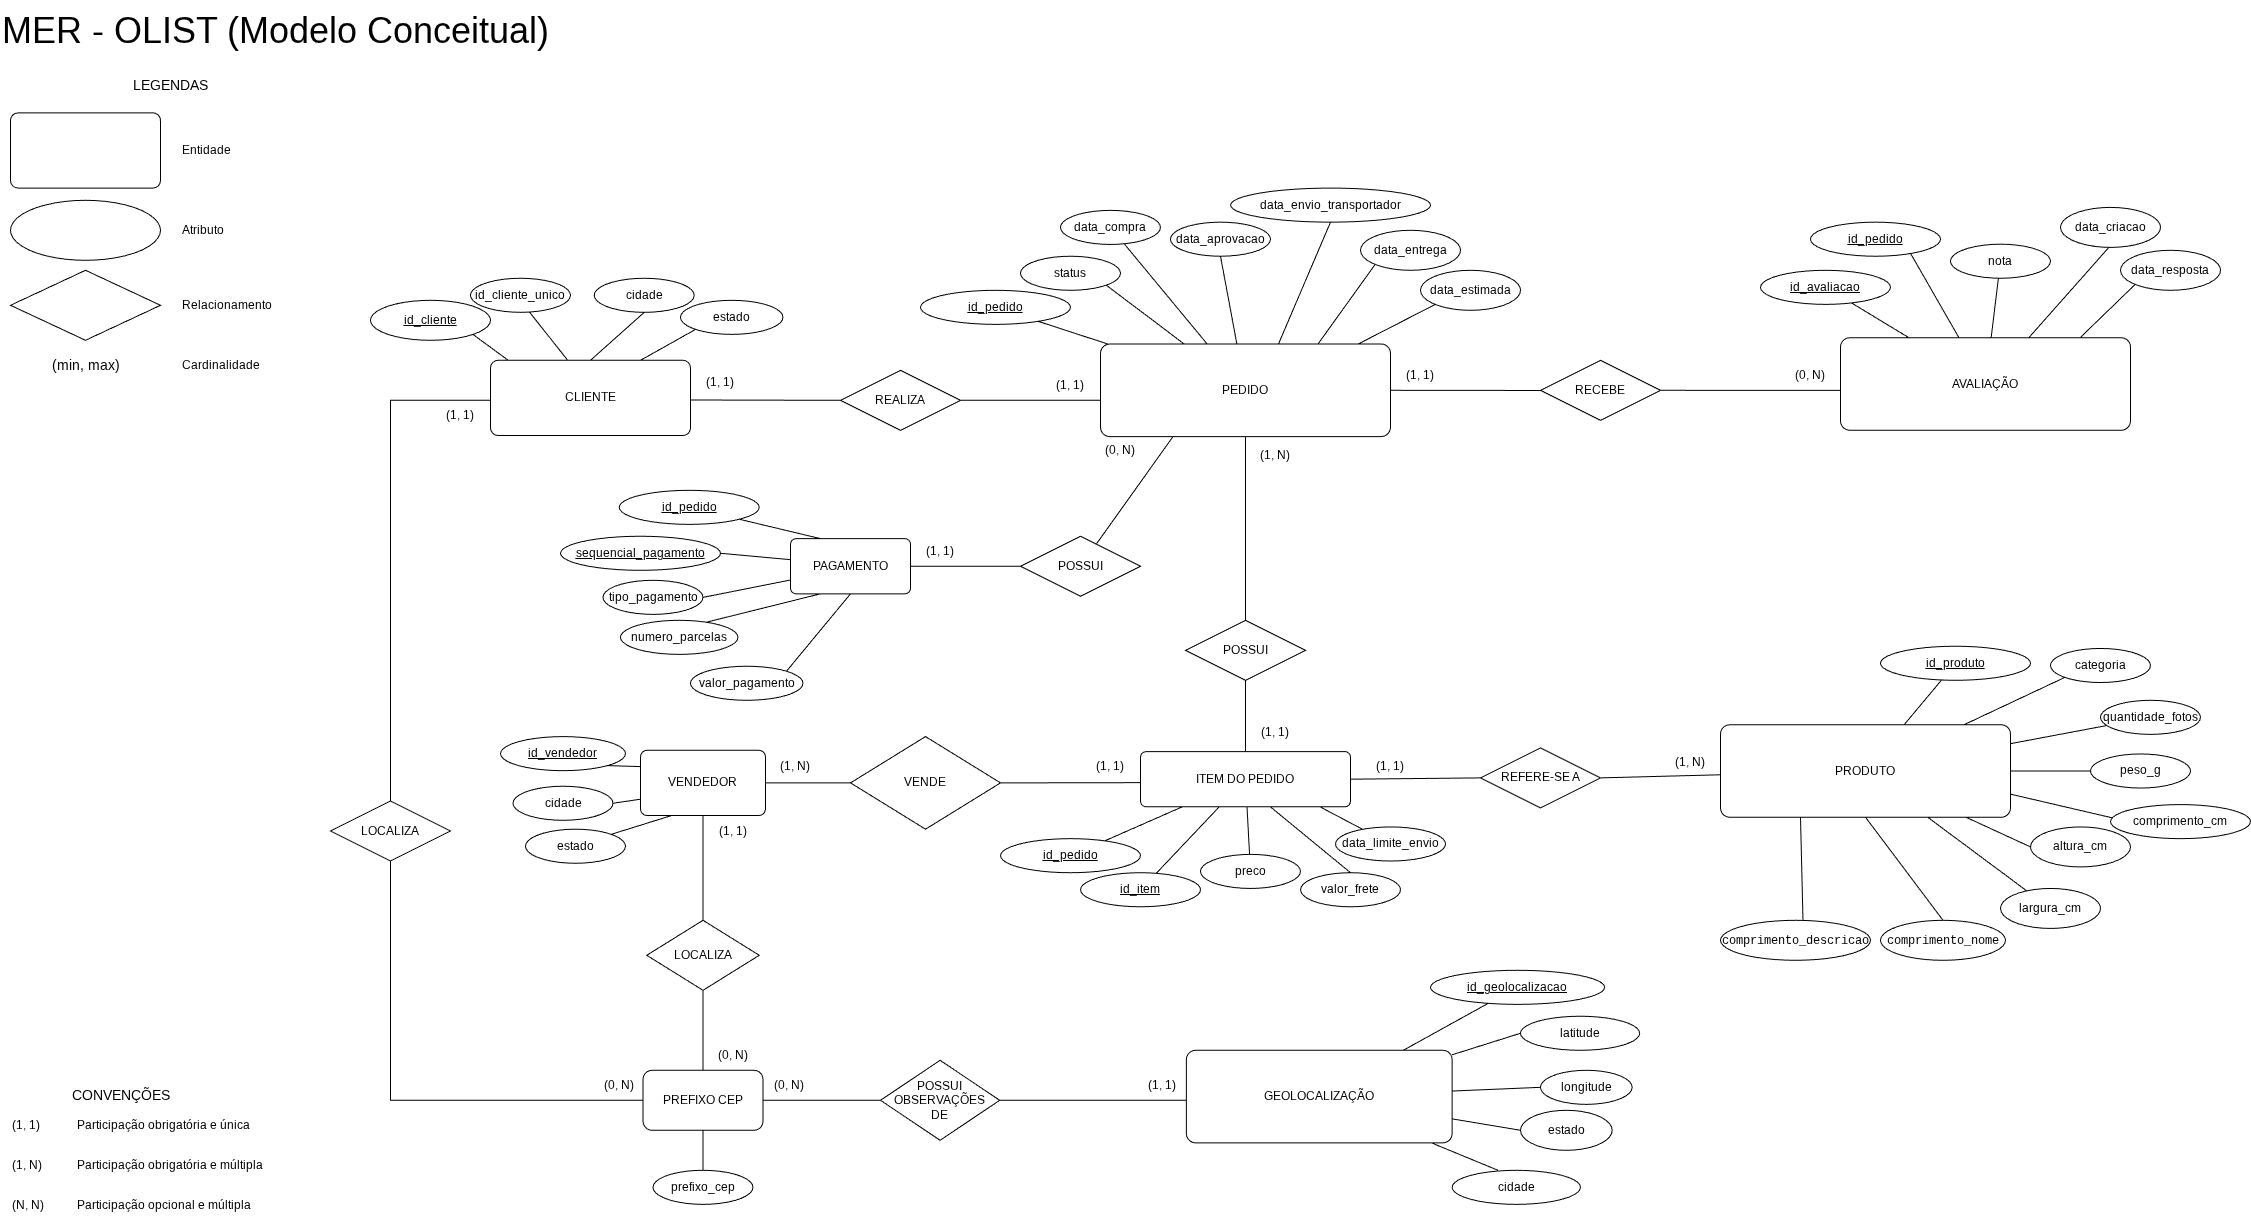
\includegraphics[
		width=\textwidth,
		height=0.78\textheight,
		keepaspectratio
		]{mer/mer-olist-conceitual.png}
		\caption{Modelo Entidade-Relacionamento conceitual consolidado.}
		\label{fig:mer-conceitual}
	\end{figure}
	
	\subsection{Resultado da Etapa}
	
	A consolidação do Modelo Entidade-Relacionamento encerra a etapa de modelagem
	conceitual do projeto.
	
	O modelo final representa nove entidades e nove relacionamentos diretos,
	preserva as diferentes granularidades identificadas no conjunto de dados e
	explicita as cardinalidades e opcionalidades consideradas adequadas ao domínio.
	
	A validação sistemática confirmou a consistência entre o diagrama, as decisões
	documentadas e as evidências obtidas durante a exploração do
	\textit{dataset}.
	
	Com a conclusão desta etapa, o MER consolidado passa a constituir a referência
	conceitual para a transformação subsequente do domínio em um modelo lógico
	relacional.
	
	% ---------------------------
	\section{Referências}
	
	\subsection{Fontes de Dados}
	
	\begin{itemize}[leftmargin=1.2cm]
		
		\item \textbf{Olist}. \\
		\textit{Brazilian E-Commerce Public Dataset by Olist}. \\
		Kaggle. Disponível em:
		\url{https://www.kaggle.com/datasets/olistbr/brazilian-ecommerce}.
		
	\end{itemize}
	
	\subsection{Referências Bibliográficas}
	
	\begin{itemize}[leftmargin=1.2cm]
		
		\item \textbf{Chen, P. P.-S.} \\
		\textit{The Entity-Relationship Model---Toward a Unified View of Data}. \\
		ACM Transactions on Database Systems, v. 1, n. 1, p. 9--36, 1976. \\
		Referência original para o Modelo Entidade-Relacionamento e para a
		representação conceitual de entidades, atributos e relacionamentos.
		
		\item \textbf{Elmasri, R.; Navathe, S.} \\
		\textit{Fundamentals of Database Systems}. \\
		Referência para conceitos de modelagem conceitual, entidades,
		atributos, relacionamentos e cardinalidades.
		
		\item \textbf{Silberschatz, A.; Korth, H.; Sudarshan, S.} \\
		\textit{Database System Concepts}. \\
		Referência para princípios de identificação, integridade,
		relacionamentos e modelagem de bancos de dados.
		
		\item \textbf{Date, C. J.} \\
		\textit{An Introduction to Database Systems}. \\
		Referência para fundamentos de bancos de dados, integridade e
		estruturação do modelo de dados.
		
	\end{itemize}
	
	\enlargethispage{2\baselineskip}
	\subsection{Ferramentas Utilizadas}
	
	\begin{itemize}[leftmargin=1.2cm]
		
		\item \textbf{diagrams.net (draw.io)}. \\
		Ferramenta utilizada para elaboração e refinamento visual do
		Modelo MER. \\
		Disponível em:
		\url{https://app.diagrams.net/}.
		
		\item \textbf{Jupyter Notebook}. \\
		Ambiente utilizado para execução das validações empíricas que
		subsidiaram decisões sobre identificadores, relacionamentos,
		cardinalidades e estrutura geográfica do modelo.
		
	\end{itemize}
	
\end{document}
